%\subsection{Choice of \acrshort{blas} Library}
\subsection{Optimized \acrshort{blas} Implementations}
\label{subseq:blas-comparison}


To perform column eliminations of a fully summed block of a frontal matrix, \acrshort{mumps} intensively calls \acrshort{gemm}, \acrshort{trsm} and \acrshort{getrf} subroutines which are parts of \acrshort{blas} and \acrshort{lapack} libraries. Figures \ref{fig:mumps:type-2-frontal-matrix} and  \ref{fig:mumps:steps-of-type-2-factorization} illustrate an application of the \acrshort{blas} subroutines to factorization of a type 2 node.\\


\figpointer{\ref{fig:mumps:type-2-frontal-matrix}}
\begin{figure}[htpb]
  \centering
  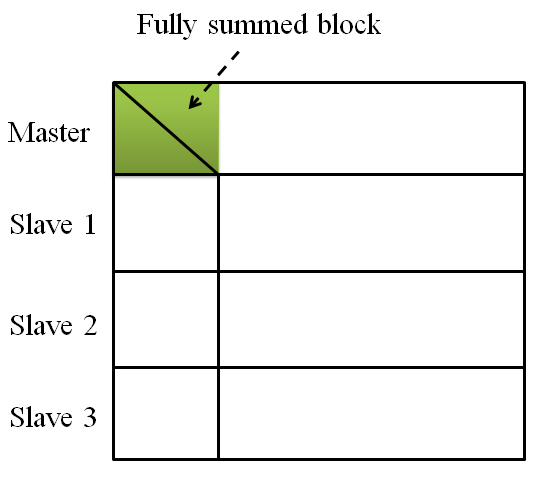
\includegraphics[width=0.45\textwidth]{figures/chapter-2/mumps-type-2-frontal-matrix.png}
\caption{One dimensional block column distribution of a type 2 node in \acrshort{mumps}}
\label{fig:mumps:type-2-frontal-matrix}
\end{figure}


\figpointer{\ref{fig:mumps:steps-of-type-2-factorization}}
\begin{figure}[htpb]
  \centering
  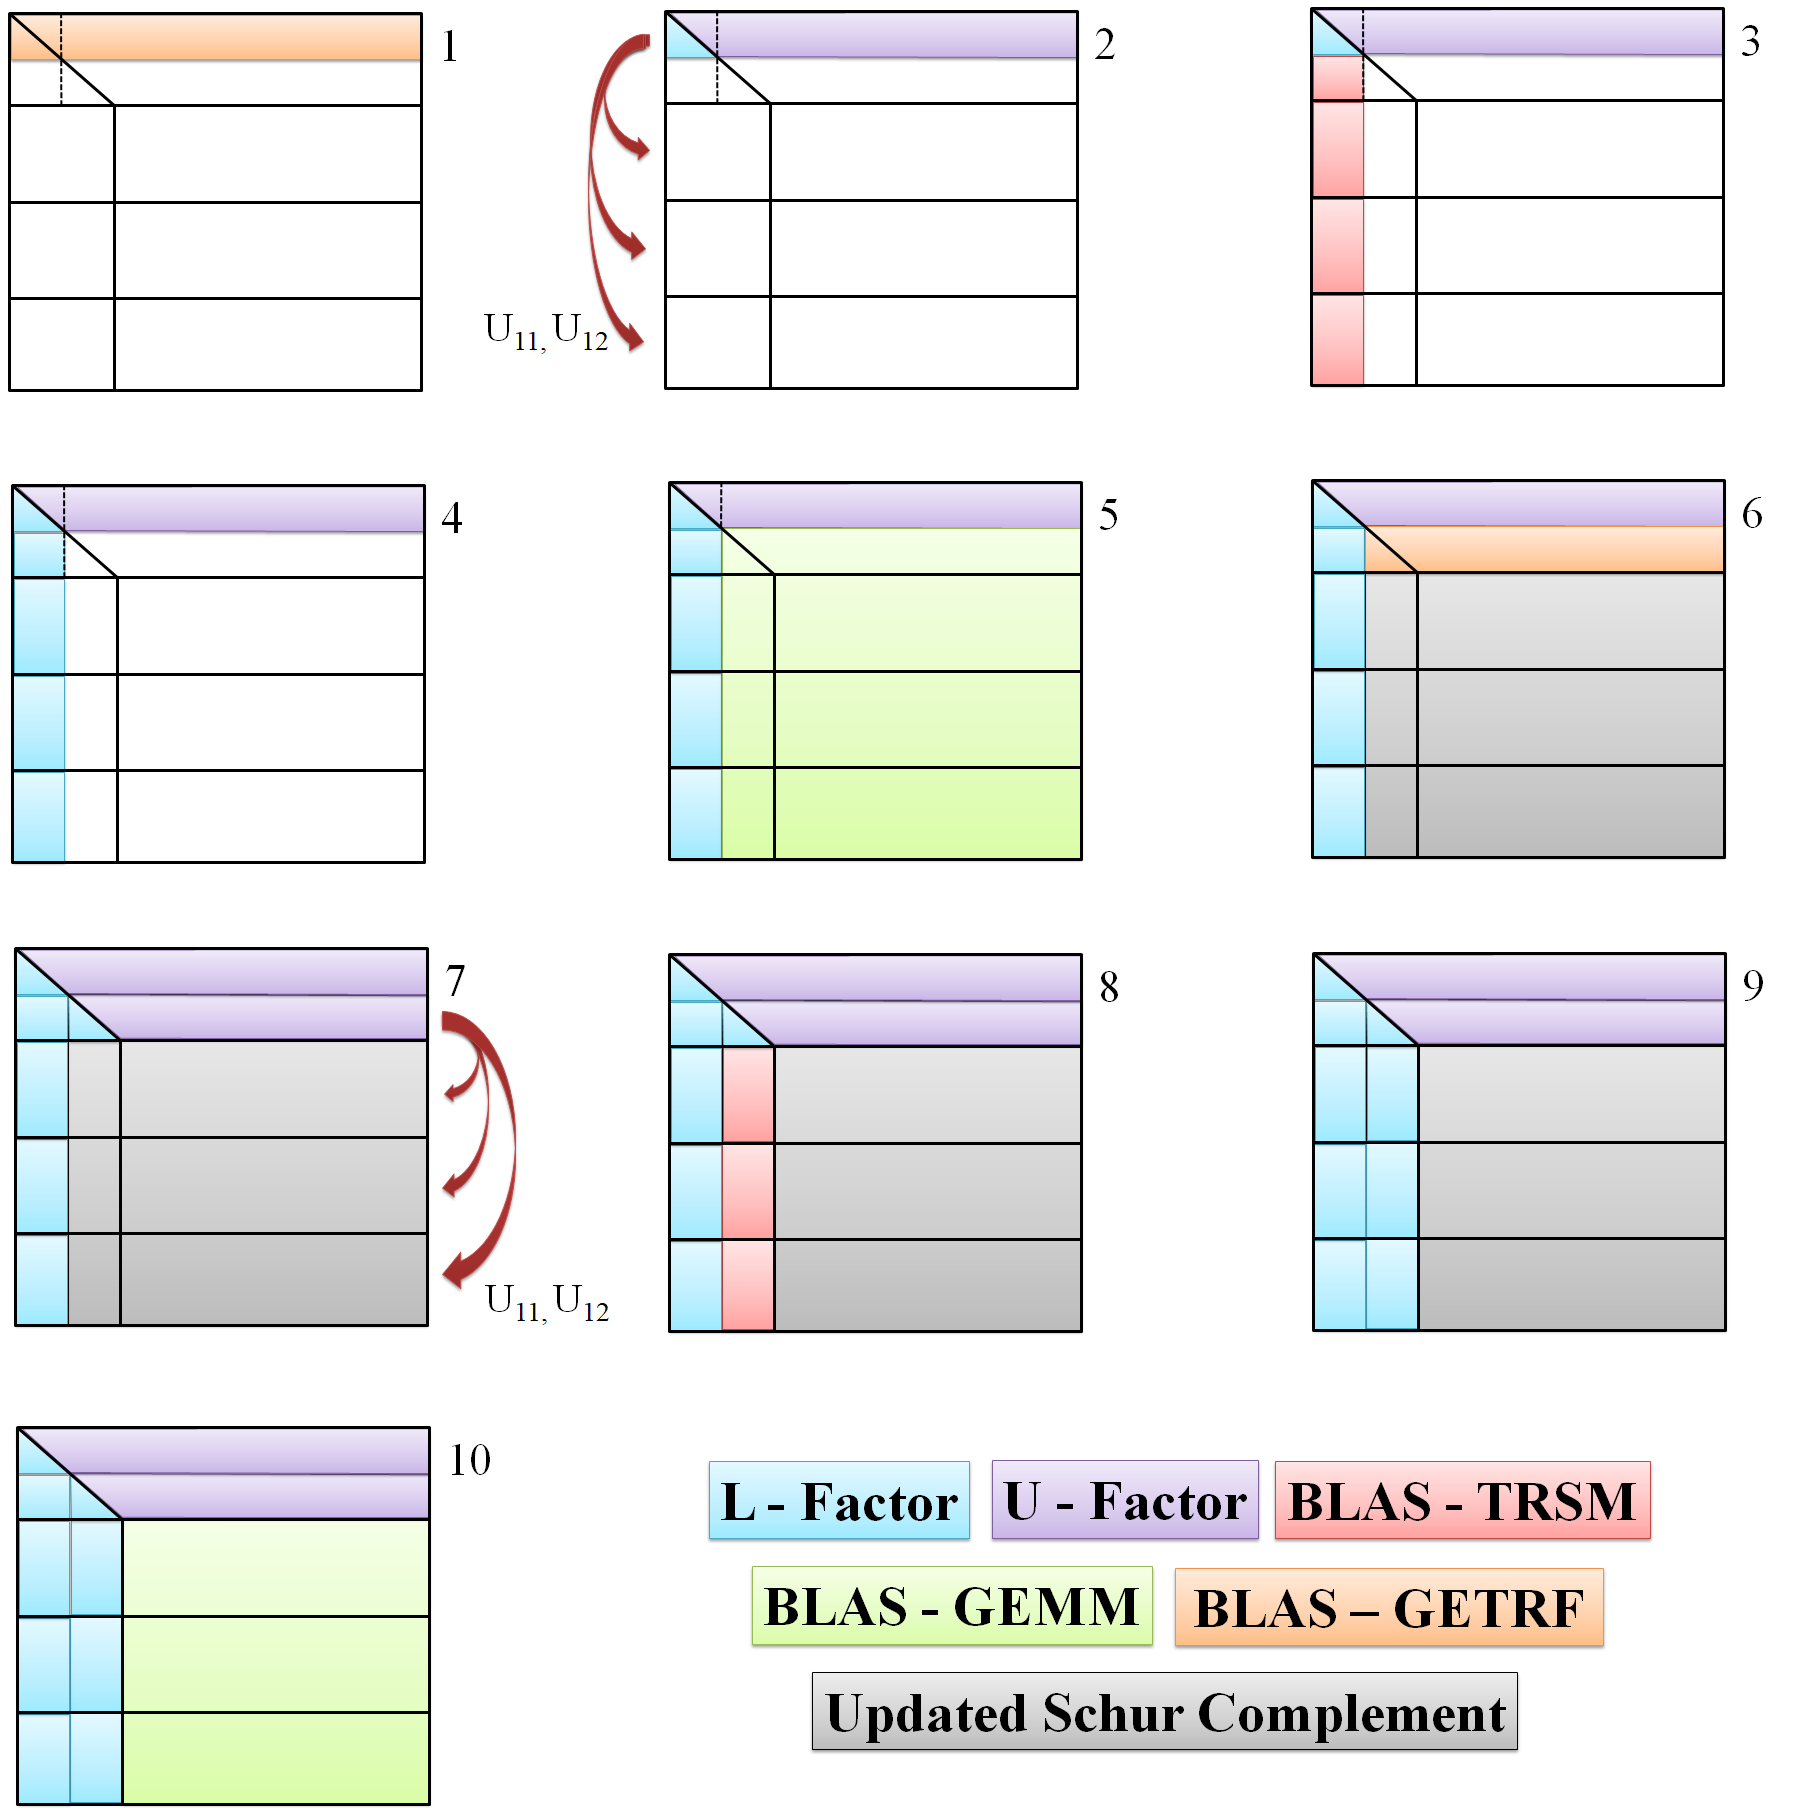
\includegraphics[width=0.85\textwidth]{figures/chapter-2/mumps-type-2-part-1.png}
\caption{An example of type 2 node factorization implemented in \acrshort{mumps}}
\label{fig:mumps:steps-of-type-2-factorization}
\end{figure}


Both \acrshort{blas} and \acrshort{lapack} libraries originate from the Netlib project which is a repository of numerous scientific computing software maintained by AT\&T Bell Laboratories, the University of Tennessee, Oak Ridge National Laboratory and other scintific communities \cite{netlib-overview}.\\


The goal of \acrshort{blas} library is provision of high efficient implementations of common dense linear algebra kernels achieved by high rates of floating point operations per memory access, low cache and Translation Lookaside Buffer (TLB) miss rates.\\


In its turn, \acrshort{lapack} is designed in such a way so that as much as possible computations are performed by calling \acrshort{blas} subroutines. This allows to achieve high efficiency for operations such as $LU$, $QR$, $SVD$ decompositions, triangular solve, etc. on modern computers. However, the Netlib \acrshort{blas} implementation is written for an abstract general-purpose central processing unit where hardware parameters are based on market statistics. Hence, it is not possible to achieve the maximum possible performance on specific hardware.\\


Therefore, there exist special-purpose, hardware-specific implementations of the library developed by hardware vendors i.e. IBM, Cray, Intel, AMD, etc., as well as open-source tuned implementations such as ATLAS, OpenBLAS, etc. To achieve full compatibility, the developers consider the Netlib implementation of \acrshort{blas} library as a standard, or a reference, and thus overwrite all its subroutines with additional tuning and optimization. This approach makes it easy to replace one \acrshort{blas} implementation by another one by substituting the corresponding object files during the linking stage. As a result, the source code of an application which calls \acrshort{blas} or \acrshort{lapack} subroutines remains the same without a need to perform any source code modifications.\\
 

Table \ref{table:list-of-blas-implementations} shows commercial and open-source tunned \acrshort{blas} implementations available on the market today.\\

\begin{table}[h!]
\centering
\small
\begin{tabular}{|c|c|c|}
\hline
Name                                                                 & Description                                                                                                                                                 & License                                                       \\ \hline
Accelerate                                                           & Apple's implementation for macOS and iOS                                                                                                                    & \begin{tabular}[c]{@{}c@{}}proprietary\\ license\end{tabular} \\ \hline
ACML                                                                 & BLAS implementation for AMD processors                                                                                                                      & \begin{tabular}[c]{@{}c@{}}proprietary\\ license\end{tabular} \\ \hline
C++ AMP                                                              & Microsoft's AMP language extension for Visual C++                                                                                                           & \begin{tabular}[c]{@{}c@{}}open\\ source\end{tabular}         \\ \hline
ATLAS                                                                & Automatically tuned BLAS implementation                                                                                                                     & \begin{tabular}[c]{@{}c@{}}open\\ source\end{tabular}         \\ \hline
Eigen BLAS                                                           & \begin{tabular}[c]{@{}c@{}}BLAS implemented on top of \\ the MPL-licensed Eigen library\end{tabular}                                                        & open source                                                   \\ \hline
ESSL                                                                 & optimized BLAS implementation for  IBM's machines                                                                                                           & \begin{tabular}[c]{@{}c@{}}proprietary\\ license\end{tabular} \\ \hline
GotoBLAS                                                             & Kazushige Goto's implementation of BLAS                                                                                                                     & \begin{tabular}[c]{@{}c@{}}proprietary\\ license\end{tabular} \\ \hline
HP MLIB                                                              & \begin{tabular}[c]{@{}c@{}}BLAS implementation supporting IA-64, PA-RISC, x86 \\ and Opteron architecture\end{tabular}                                      & \begin{tabular}[c]{@{}c@{}}proprietary\\ license\end{tabular} \\ \hline
Intel MKL                                                            & \begin{tabular}[c]{@{}c@{}}Intel's implementation of BLAS optimized for\\ Intel Pentium, Core,  Xeon and Xeon Phi\end{tabular}                              & \begin{tabular}[c]{@{}c@{}}proprietary\\ license\end{tabular} \\ \hline
Netlib BLAS                                                          & The official reference implementation on Netlib                                                                                                             & \begin{tabular}[c]{@{}c@{}}open\\ source\end{tabular}         \\ \hline
OpenBLAS                                                             & Optimized BLAS library based on GotoBLAS                                                                                                                    & \begin{tabular}[c]{@{}c@{}}open\\ source\end{tabular}         \\ \hline
PDLIB/SX                                                             & BLAS library targeted to the NEC SX-4 system                                                                                                                & \begin{tabular}[c]{@{}c@{}}proprietary\\ license\end{tabular} \\ \hline
SCSL                                                                 & BLAS implementations for SGI's Irix workstations                                                                                                            & \begin{tabular}[c]{@{}c@{}}proprietary\\ license\end{tabular} \\ \hline
\begin{tabular}[c]{@{}c@{}}Sun\\ Performance \\ Library\end{tabular} & \begin{tabular}[c]{@{}c@{}}Optimized BLAS and LAPACK for SPARC, Core \\ and AMD64 architectures under \\ Solaris 8, 9, and 10 as well as Linux\end{tabular} & \begin{tabular}[c]{@{}c@{}}proprietary\\ license\end{tabular} \\ \hline
\end{tabular}
\caption{Commercial and open source \acrshort{blas} libraries \cite{wiki:blas-implementations}}
\label{table:list-of-blas-implementations}
\end{table}



Among all libraries listed in table \ref{table:list-of-blas-implementations} there were only four available in \gls{hw1} machine environment, namely: Netlib \acrshort{blas}, Intel MKL, OpenBLAS and ATLAS. However, installation of ATLAS requires to switch off dynamic frequency scaling, also called CPU throttling, to allow ATLAS configuration routines to find the best loop transformation parameters for specific hardware. In order to turn off CPU throttling, one has to reboot the entire machine and make appropriate changes in Basic Input/Output System (BIOS). This fact made ATLAS library not suitable for the study and we excluded it from our primary list of candidates. Moreover, during installation, one has to explicitly specify the number of \acrshort{openmp} threads that are going to be forked once a \acrshort{blas} subroutine is called. This means there is no way to change the number of threads per \acrshort{mpi} process in run-time without re-installation of the library. Thus, only 3 versions of \acrshort{mumps}-\acrshort{petsc} (linked with Netlib \acrshort{blas}, Intel MKL and OpenBLAS) library were compiled, installed and tested using both \acrshort{grs} and SuiteSparse matrix sets and 1 thread per \acrshort{mpi} process i.e. flat-\acrshort{mpi} mode. Results of testing were obtained on \gls{hw1} machine and are represented in figures \ref{fig:mumps-blas-configuration-1}, \ref{fig:mumps-blas-configuration-2} and appendix \ref{app:app-blas-configuration}.\\


\figpointer{\ref{fig:mumps-blas-configuration-1}}
\begin{figure}[htpb]
\centering
	\begin{tabular}{cc}
		\subfloat[k3-18]{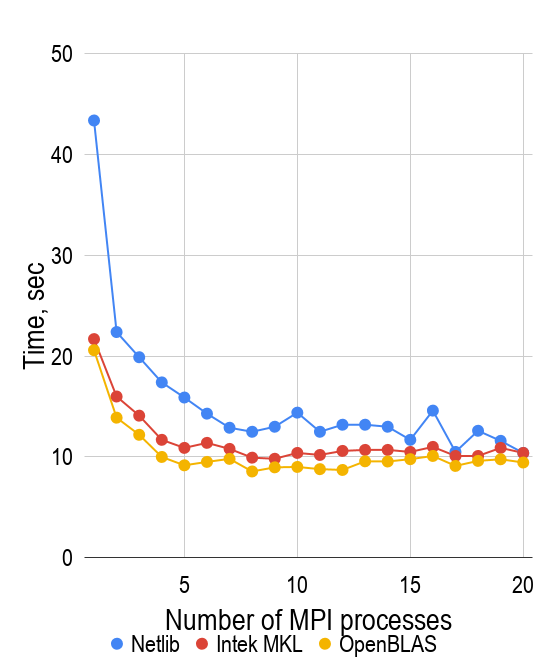
\includegraphics[width=0.48\textwidth]{figures/chapter-2/blas-configuration/k3-18.png}} &
		\subfloat[cube-645]{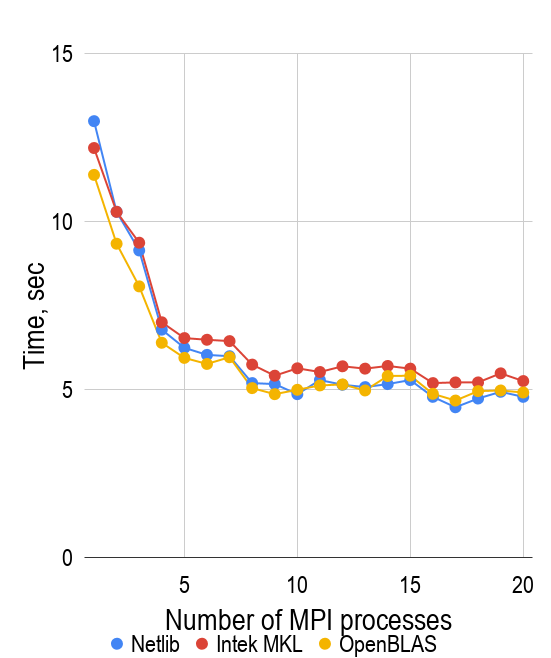
\includegraphics[width=0.48\textwidth]{figures/chapter-2/blas-configuration/cube-645.png}} \\
		\subfloat[k3-2]{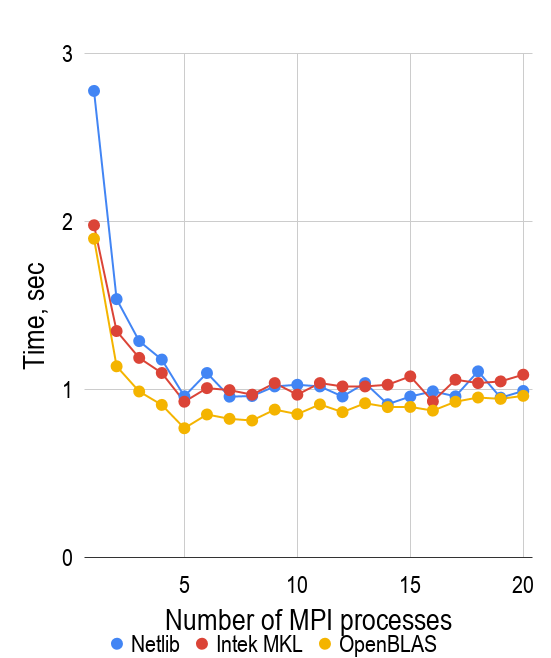
\includegraphics[width=0.48\textwidth]{figures/chapter-2/blas-configuration/k3-2.png}} &
		\subfloat[cube-64]{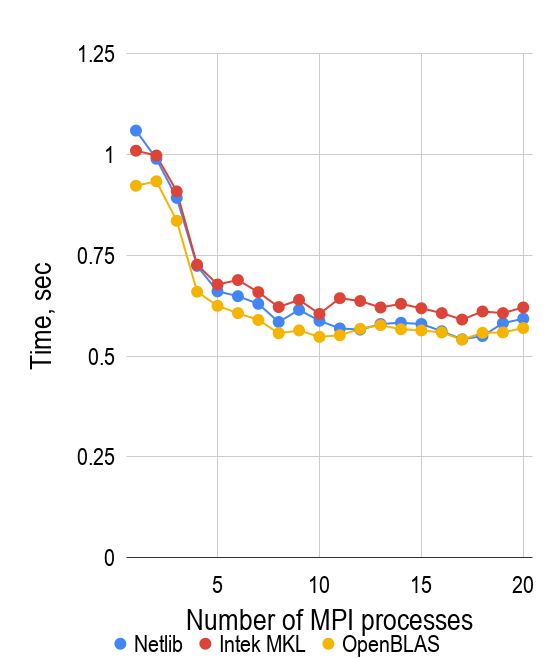
\includegraphics[width=0.48\textwidth]{figures/chapter-2/blas-configuration/cube-64.png}} \\
	\end{tabular}
	\caption{Comparisons of parallel factorization of \acrshort{grs} matrix set performed on \gls{hw1} machine using  MUMPS solver linked to different \acrshort{blas} implementations}
	\label{fig:mumps-blas-configuration-1}
\end{figure}


\figpointer{\ref{fig:mumps-blas-configuration-2}}
\begin{figure}[htpb]
\centering
	\begin{tabular}{cc}
		\subfloat[cube-5]{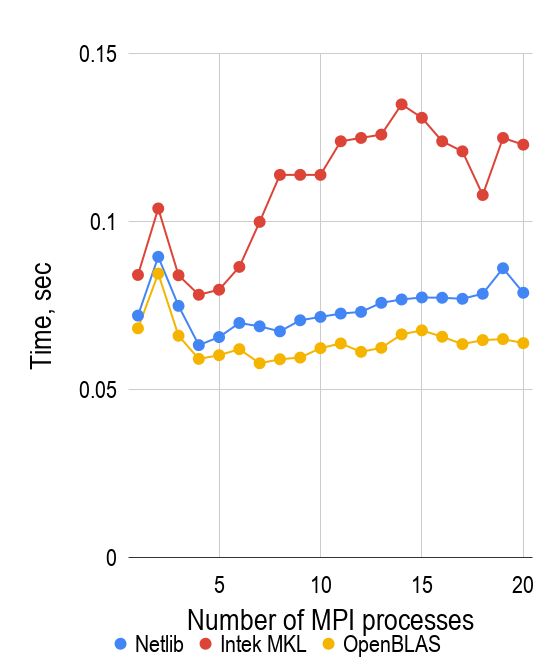
\includegraphics[width=0.43\textwidth]{figures/chapter-2/blas-configuration/cube-5.png}} &
		\subfloat[pwr-3d]{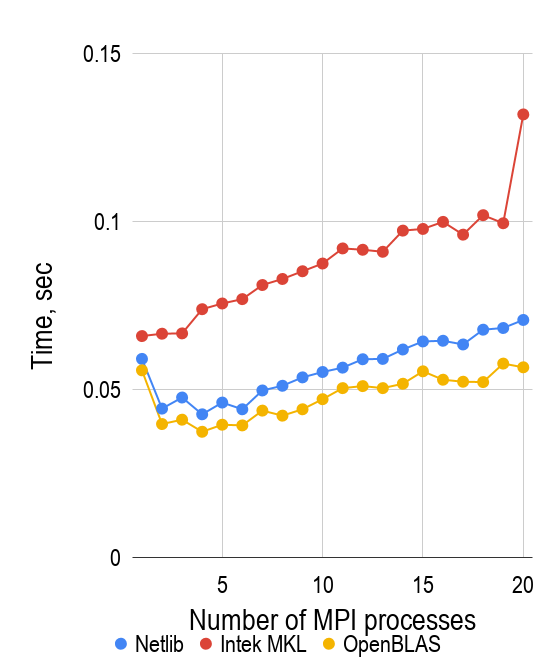
\includegraphics[width=0.43\textwidth]{figures/chapter-2/blas-configuration/pwr-3d.png}} \\
		\subfloat[PFlow\_742]{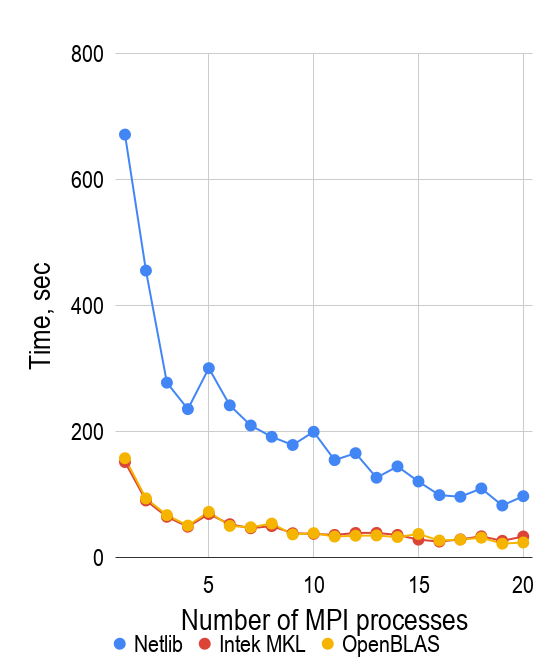
\includegraphics[width=0.48\textwidth]{figures/chapter-2/blas-configuration/PFlow_742.png}} & \subfloat[torso3]{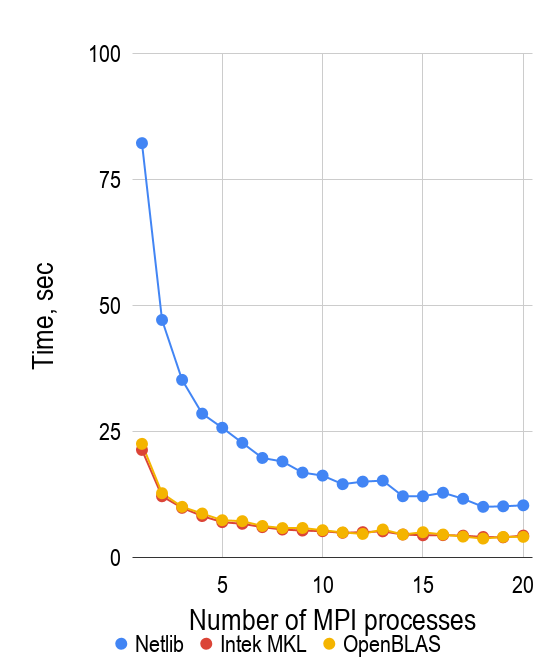
\includegraphics[width=0.48\textwidth]{figures/chapter-2/blas-configuration/torso3.png}} \\
	\end{tabular}
	\caption{Comparisons of parallel factorizations of \acrshort{grs} and SuiteSparse matrix sets performed on \gls{hw1} machine using  MUMPS solver linked to different \acrshort{blas} implementations}
	\label{fig:mumps-blas-configuration-2}
\end{figure}



The tests show that OpenBLAS outperforms both Netlib and Intel MKL libraries in case of \acrshort{grs} matrix set. On average, OpenBLAS is about \textbf{13\%} faster than the default Netlib implementation and approximately \textbf{21\%} faster than Intel MKL library. It is interesting to notice Intel MKL library turns out to be slower than the default Netlib \acrshort{blas} implementation for small- and medium-sized \acrshort{grs} matrices in almost \textbf{52\%} and \textbf{2\%}, respectively. At the same time, both tuned libraries, OpenBLAS and Intel MKL, show significant performance gain in comparison to the standard Netlib \acrshort{blas} implementation in case of SuiteSparse matrix set. The libraries reduce the execution time by almost \textbf{50\%} on an average. In opposite to \acrshort{grs} matrix set, it turns out that Intel MKL is often faster than OpenBLAS for almost all test-cases from SuiteSparse matrix set. However, the difference between them is negligibly small. The result of the comparison are summarized in tables \ref{table:mumps-blas-performance-gain-grs} and \ref{table:mumps-blas-performance-gain-suitesprase}.\\


\begin{table}[h!]
\centering
\begin{tabular}{|c|c|c|c|}
\hline
\begin{tabular}[c]{@{}c@{}}Matrix\\ Name\end{tabular} & \begin{tabular}[c]{@{}c@{}}Performance\\ gain of \\ OpenBLAS \\ relatively to \\ Netlib \%\end{tabular} & \begin{tabular}[c]{@{}c@{}}Performance\\ gain of\\ IntelMKL\\ relatively to\\ Netlib \%\end{tabular} & \begin{tabular}[c]{@{}c@{}}Performance\\ gain of\\ OpenBLAS\\ relatively to\\ Intel MKL \%\end{tabular} \\ \hline
pwr-3d                                                & 14.607                                                                                                  & -56.249                                                                                              & 44.695                                                                                                  \\ \hline
cube-5                                                & 13.569                                                                                                  & -47.797                                                                                              & 39.931                                                                                                  \\ \hline
cube-64                                               & 4.385                                                                                                   & -5.483                                                                                               & 9.323                                                                                                   \\ \hline
cube-645                                              & 1.897                                                                                                   & -7.474                                                                                               & 8.702                                                                                                   \\ \hline
k3-2                                                  & 13.906                                                                                                  & 0.833                                                                                                & 13.057                                                                                                  \\ \hline
k3-18                                                 & 29.914                                                                                                  & 21.03                                                                                                & 11.29                                                                                                   \\ \hline
\end{tabular}
\caption{Comparisons of different \acrshort{mumps}-\acrshort{blas} configurations applied to \acrshort{grs} matrix set}
\label{table:mumps-blas-performance-gain-grs}
\end{table}



\begin{table}[h!]
\centering
\begin{tabular}{|c|c|c|c|}
\hline
\begin{tabular}[c]{@{}c@{}}Matrix\\ Name\end{tabular} & \begin{tabular}[c]{@{}c@{}}Performance\\ gain of \\ OpenBLAS \\ relatively to \\ Netlib \%\end{tabular} & \begin{tabular}[c]{@{}c@{}}Performance\\ gain of\\ IntelMKL\\ relatively to\\ Netlib \%\end{tabular} & \begin{tabular}[c]{@{}c@{}}Performance\\ gain of\\ OpenBLAS\\ relatively to\\ Intel MKL \%\end{tabular} \\ \hline
cant                                                  & 26.981                                                                                                  & 25.964                                                                                               & 1.233                                                                                                   \\ \hline
consph                                                & 67.617                                                                                                  & 68.252                                                                                               & -2.327                                                                                                  \\ \hline
CurlCurl\_3                                           & 78.804                                                                                                  & 79.37                                                                                                & -3.371                                                                                                  \\ \hline
Geo\_1438                                             & 83.106                                                                                                  & 83.565                                                                                               & -2.857                                                                                                  \\ \hline
memchip                                               & 6.066                                                                                                   & -6.909                                                                                               & 11.883                                                                                                  \\ \hline
PFlow\_742                                            & 75.574                                                                                                  & 74.943                                                                                               & 1.416                                                                                                   \\ \hline
pkustk10                                              & 35.089                                                                                                  & 34.536                                                                                               & 0.502                                                                                                   \\ \hline
torso3                                                & 66.185                                                                                                  & 66.988                                                                                               & -2.837                                                                                                  \\ \hline
x104                                                  & 41.82                                                                                                   & 41.936                                                                                               & -0.445                                                                                                  \\ \hline
\end{tabular}
\caption{Comparisons of different \acrshort{mumps}-\acrshort{blas} configurations applied to SuiteSparse matrix set}
\label{table:mumps-blas-performance-gain-suitesprase}
\end{table}


It can be clearly observed from the tables that test-cases derived from \acrshort{grs} matrix set demonstrate insignificant improvements in execution time in constant to the tests generated with SuiteSparse matrix set. This may be explained by relatively small numbers of type 2 nodes in assembly trees resulted from \acrshort{grs} test-cases. In this case, the trees are mainly formed by the root and type 1 nodes. As it was mentioned in subsection \ref{subseq:mumps-review}, type 1 nodes are grouped in subtrees and each subtree is processed by a single \acrshort{mpi} process. According to the documentation, it is not clear whether \acrshort{mumps} calls \acrshort{blas} subroutines while processing a type 1 node. Even if it is a case performance of \acrshort{blas} can be limited because of small sizes of frontal matrices of such nodes.\\

We assume that, in the general case, lack of type 2 nodes in an assembly tree can be due to an inefficient amalgamation process of the corresponding elimination tree resulted from the matrix sparsity pattern.\\


Based on the obtained results, comparisons between different matrix sets and our reasoning, we presume that \acrshort{athlet} generates linear systems resulting in such trees where type 1 nodes predominate over the others. We can assume it is due to specifics of numerical spacial and time integration explained in section \ref{sec:athlet-overview}.\\


In this subsection, we have shown where and how \acrshort{mumps} utilizes \acrshort{blas} and \acrshort{lapack} libraries. We have compared two tuned \acrshort{blas} implementations with a baseline, Netlib \acrshort{blas}, using two different matrix sets. We have shown the overall statistics of the obtained results and come to the conclusion that \acrshort{mumps}-OpenBLAS configuration is the best one for \acrshort{grs} matrix set. Additionally, we have given reasoning for a noticeable difference between results obtained from different matrix sets as well as we have talked about probable specifics of linear systems generated by \acrshort{athlet}.\\
